\documentclass[10pt]{beamer}

\usetheme{metropolis}
\usepackage{appendixnumberbeamer}
\usepackage{booktabs}
\usepackage[scale=2]{ccicons}
\usepackage{pgfplots}
\usepackage{color}
\usepgfplotslibrary{dateplot}
\usepackage{xspace}
\newcommand{\themename}{\textbf{\textsc{metropolis}}\xspace}

\usepackage{stmaryrd}
\usepackage{amsmath}
\usepackage{verbatim}
\usepackage{tikz}
\usetikzlibrary{shapes}
\usepackage{siunitx}
\usepackage{color}
\usepackage[normalem]{ulem}
\usetikzlibrary{calc,decorations.pathmorphing,patterns}
\usepackage{amssymb}
\usepackage{amsfonts}
\usepackage{amscd}
\usepackage{amsthm}
\usepackage{mathrsfs}
\usepackage{enumerate}
\usepackage{mathtools}
\usepackage{booktabs}
\usepackage{array}
\usepackage{nth}
\usepackage{lipsum}


%%%%%%%%%%%%%%%%%%%%%%%%%%%%%list %%%%%%%%%%%%%%%%%
\usepackage{textcomp}           % To use with matlab-prettifier
\usepackage{listings}
\usepackage[framed , numbered]{matlab-prettifier}
\usepackage{listings}
%%%%%%%%%%%%%%%%%end of list%%%%%%%%%%%%%%%%%%%%%

%%%%%%%%%%%%%%%%%%%%%%%%%%%%%%%%%%%%%%%%%%%%%%%%%%%%%%%%%%%%%%%%%%%%%%%%%
%%%% The following is for fancy box %%%%%%%%%%%%%%
\usepackage[framemethod=TikZ]{mdframed}
%%%%%%%%%%%%% Theorem %%%%%%%%%%%%
\newenvironment{thm}[2][]{%
\ifstrempty{#1}%
{\mdfsetup{%
frametitle={%
\tikz[baseline=(current bounding box.east),outer sep=0pt]
\node[anchor=east,rectangle,fill=red!20]
{\strut Theorem};}}
}%
{\mdfsetup{%
frametitle={%
\tikz[baseline=(current bounding box.east),outer sep=0pt]
\node[anchor=east,rectangle,fill=red!20]
{\strut Theorem #1};}}%
}%
\mdfsetup{innertopmargin=1pt,linecolor=red!20,%
linewidth=2pt,topline=true,%
frametitleaboveskip=\dimexpr-\ht\strutbox\relax
}
\begin{mdframed}[]\relax%
\label{#2}}{\end{mdframed}}
%%%%%%%%%%%%%%Lemma%%%%%%%%%%%%%%%%%%%%%%%%%%%%%%%%%%%%%%%%%%%%%%%%%%%%%%
\newcounter{lem}[section] \setcounter{lem}{0}
\renewcommand{\thelem}{}
\newenvironment{lem}[2][]{%
\refstepcounter{lem}%
\ifstrempty{#1}%
{\mdfsetup{%
frametitle={%
\tikz[baseline=(current bounding box.east),outer sep=0pt]
\node[anchor=east,rectangle,fill=green!20]
{\strut Lemma~\thelem};}}
}%
{\mdfsetup{%
frametitle={%
\tikz[baseline=(current bounding box.east),outer sep=0pt]
\node[anchor=east,rectangle,fill=green!20]
{\strut Lemma~\thelem:~#1};}}%
}%
\mdfsetup{innertopmargin=1pt,linecolor=green!20,%
linewidth=2pt,topline=true,%
frametitleaboveskip=\dimexpr-\ht\strutbox\relax
}
\begin{mdframed}[]\relax%
\label{#2}}{\end{mdframed}}
%%%%%%%%%%%%%%%%%%%%%%%%%%%%%%%%%%%%%%%%%%%%%%%%%%%%%%%%%%%%%%%%%%%%%%%
%Corollary
\newenvironment{cor}[2][]{%
\ifstrempty{#1}%
{\mdfsetup{%
frametitle={%
\tikz[baseline=(current bounding box.east),outer sep=0pt]
\node[anchor=east,rectangle,fill=blue!30]
{\strut Corollary};}}
}%
{\mdfsetup{%
frametitle={%
\tikz[baseline=(current bounding box.east),outer sep=0pt]
\node[anchor=east,rectangle,fill=blue!30]
{\strut Corollary:~#1};}}%
}%
\mdfsetup{innertopmargin=1pt,linecolor=blue!30,%
linewidth=2pt,topline=true,%
frametitleaboveskip=\dimexpr-\ht\strutbox\relax
}
\begin{mdframed}[]\relax%
\label{#2}}{\end{mdframed}}
%%%%%%%%%%%%%%%%%%%%%%%%%%%%%%%%%%%%%%%%%%%%%%%%%%%%%%%%%%%%%%%%%%%%%%%
%Proof
\newenvironment{prove}[2][]{%
\ifstrempty{#1}%
{\mdfsetup{%
frametitle={%
\tikz[baseline=(current bounding box.east),outer sep=0pt]
\node[anchor=east,rectangle,fill=red!20]
{\strut Proof};}}
}%
{\mdfsetup{%
frametitle={%
\tikz[baseline=(current bounding box.east),outer sep=0pt]
\node[anchor=east,rectangle,fill=red!20]
{\strut Proof:~#1};}}%
}%
\mdfsetup{innertopmargin=1pt,linecolor=red!20,%
linewidth=2pt,topline=true,%
frametitleaboveskip=\dimexpr-\ht\strutbox\relax
}
\begin{mdframed}[]\relax%
\label{#2}}{\end{mdframed}}
%%%%%%%%%%%%%%%%%%%%%%%%%%%%%%%%%%%%%%%%%%%%%%%%%%%%%%%%%%%%%%%%%%%%%%%
%Defintion
\newcounter{drf}[section]\setcounter{drf}{0}
\renewcommand{\thedrf}{}
\newenvironment{drf}[2][]{%
\refstepcounter{drf}%
\ifstrempty{#1}%
{\mdfsetup{%
frametitle={%
\tikz[baseline=(current bounding box.east),outer sep=0pt]
\node[anchor=east,rectangle,fill=orange!20]
{\strut Definition~\thedrf};}}
}%
{\mdfsetup{%
frametitle={%
\tikz[baseline=(current bounding box.east),outer sep=0pt]
\node[anchor=east,rectangle,fill=orange!20]
{\strut Definition~\thedrf:~#1};}}%
}%
\mdfsetup{innertopmargin=1pt,linecolor=orange!20,%
linewidth=2pt,topline=true,%
frametitleaboveskip=\dimexpr-\ht\strutbox\relax
}
\begin{mdframed}[]\relax%
\label{#2}}{\end{mdframed}}
%%%%%%%%%%%%%%%%%%%%%%%%%%%%%%%%%%%%%%%%%%%%%%%%%%%%%%%%%%%%%%%%%%%%%%%%%%%
% end of self defined label
%%%%%%%%%%%%%%%%%%%%%%%%%%%%%%%%%%%%%%%%%%%%%%%%%%%%%%%%%%%%%%%%%%%%%%%%%%%


%%%%%%%%%%%%%% For double curly bracket%%%%%%%%%%%%%%%%
\usepackage{xparse}

\NewDocumentCommand{\dgal}{sO{}m}{%
  \IfBooleanTF{#1}
    {\dgalext{#3}}
    {\dgalx[#2]{#3}}%
}

\NewDocumentCommand{\dgalext}{m}{%
  \sbox0{%
    \mathsurround=0pt % just for safety
    $\left\{\vphantom{#1}\right.\kern-\nulldelimiterspace$%
  }%
  \sbox2{\{}%
  \ifdim\ht0=\ht2
    \{\kern-.45\wd2 \{#1\}\kern-.45\wd2 \}%
  \else
    \left\{\kern-.5\wd0\left\{#1\right\}\kern-.5\wd0\right\}%
  \fi
}

\NewDocumentCommand{\dgalx}{om}{%
  \sbox0{\mathsurround=0pt$#1\{$}%
  \sbox2{\{}%
  \ifdim\ht0=\ht2
    \{\kern-.45\wd2 \{#2\}\kern-.45\wd2 \}%
  \else
    \mathopen{#1\{\kern-.5\wd0 #1\{}
    #2
    \mathclose{#1\}\kern-.5\wd0 #1\}}
  \fi
}
%%%%%%%%%%%%%%%%



%%%%%%%%%%%%%%%%%%%%%%%%%%%%%%%%%%%%%

\usepackage{animate}

\graphicspath{{./fig/}}


%%%%%%%%%%%%%% define color %%%%%%%%%%%%%%%%%%
\definecolor{DarkFern}{HTML}{407428}
\definecolor{DarkCharcoal}{HTML}{4D4944}
\colorlet{Fern}{DarkFern!85!white}
\colorlet{Charcoal}{DarkCharcoal!85!white}
\colorlet{LightCharcoal}{Charcoal!50!white}
\colorlet{AlertColor}{orange!80!black}
\colorlet{DarkRed}{red!70!black}
\colorlet{DarkBlue}{blue!70!black}
\colorlet{DarkGreen}{green!70!black}

\newcommand{\I}{\mathrm{i}}




%%%%%%%%%%%%%%%%%%%%%%%%%%%%%%%%%%%%%%
%\newcommand{\G}{\alert{G}}  % change color of main author



%%%%%%%%%%%%% Title Page %%%%%%%%%%%%%%%%%%%

\title{MAST90026 Computational Differential\\Equations: Week 5}
%\subtitle{A modern beamer theme}
\date{Semester 1 2024}
\author{Jesse Collis\\Modified from Hailong Guo (2022)}
\institute{The University of Melbourne}
\titlegraphic{\vspace{6cm}\flushright\includegraphics[height=2cm]{logo.png}}


\begin{document}

\maketitle


%
%
%\begin{frame}{Table of contents}
%  \setbeamertemplate{section in toc}[sections numbered]
%  \tableofcontents[hideallsubsections]
%\end{frame}


%-=-=-=-=-=-=-=-=-=-=-=-=-=-=-=-=-=-=-=-=-=-=-=-=
%
%	SECTION: 
%
%-=-=-=-=-=-=-=-=-=-=-=-=-=-=-=-=-=-=-=-=-=-=-=-=
%\section{Method of Weighted Residuals}





%-=-=-=-=-=-=-=-=-=-=-=-=-=-=-=-=-=-=-=-=-=-=-=-=
%	FRAME:
%-=-=-=-=-=-=-=-=-=-=-=-=-=-=-=-=-=-=-=-=-=-=-=-=
\begin{frame}{Classification of 2nd order partial differential equations}


A linear second order partial differential equation can be written as
$$
A u_{x x}+B u_{x y}+C u_{y y}=F\left(x, y, u, u_{x}, u_{y}\right)
$$
where $A, B$ and $C$ may be functions of $x$ and $y$. Based on the local value of the coefficients the equations are classified as follows:
$$
\begin{array}{ll}
B^{2}-4 A C>0 & \text { Hyperbolic } \\
B^{2}-4 A C=0 & \text { Parabolic } \\
B^{2}-4 A C<0 & \text { Elliptic }
\end{array}
$$


\alert{Example}
\begin{align*}
-\nabla^2u&=f, &&\mbox{The Poisson equation, elliptic,}\\
\nabla^2u&=u_t, &&\mbox{The diffusion equation, parabolic,}\\
\nabla^2u&=u_{tt}, &&\mbox{The wave equation, hyperbolic.}
\end{align*}

\end{frame}



%-=-=-=-=-=-=-=-=-=-=-=-=-=-=-=-=-=-=-=-=-=-=-=-=
%	FRAME:
%-=-=-=-=-=-=-=-=-=-=-=-=-=-=-=-=-=-=-=-=-=-=-=-=
\begin{frame}{Elliptic equation}
Consider (a subclass of) the elliptic PDEs:
\begin{equation*}
-\nabla \cdot (D(x,y)\nabla u)=f(x,y),
\end{equation*}
where $D>0$  to satisfy ellipticity.

\vspace{1em}
Possible boundary conditions:
\begin{itemize}
	\item Dirichelt BC: $u=g_D(x,y) \text{  on } \partial \Omega$.
	\item Neumann BC: $q\cdot \vec{n}=g_N(x,y)  \text{  on } \partial \Omega$
	\item Robin BC: $\alpha u +\beta q\cdot \vec{n}=g_R \text{ on } \partial \Omega$
\end{itemize}
where $q = -D(x,y)\nabla u$.

\end{frame}
   

%-=-=-=-=-=-=-=-=-=-=-=-=-=-=-=-=-=-=-=-=-=-=-=-=
%	FRAME:
%-=-=-=-=-=-=-=-=-=-=-=-=-=-=-=-=-=-=-=-=-=-=-=-=
\begin{frame}{Discretisation of domain }
Questions:
\begin{itemize}
\item How to handle the curved boundaries?
\item How to define the mesh in 2D?
\end{itemize}



\vspace{1em}
\alert{To avoid the problem},  considering a rectangle aligned with the axes. In addition, we consider Poisson equation by assuming $D=1$. 

\end{frame}
   



%-=-=-=-=-=-=-=-=-=-=-=-=-=-=-=-=-=-=-=-=-=-=-=-=
%	FRAME:
%-=-=-=-=-=-=-=-=-=-=-=-=-=-=-=-=-=-=-=-=-=-=-=-=
\begin{frame}{Poisson equation in 2D }

\begin{columns}


\begin{column}{.4\textwidth}
\begin{align*}
	-\nabla^2 u(x, y) &= f(x, y), \quad \text{ in } \Omega,\\
	                 u &= g_D,    \quad\quad \,\,\,\,\,  \text{ on } \partial \Omega.
\end{align*}


\begin{equation*}
	\nabla^2 \equiv \frac{\partial^2}{\partial x^2}
	+ \frac{\partial^2}{\partial y^2}
\end{equation*}

\end{column}

\begin{column}{.6\textwidth}
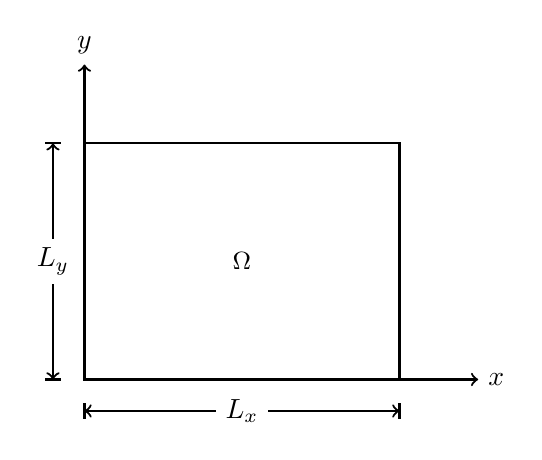
\begin{tikzpicture}




 
 
   

 \draw [black, thick] (0,0) rectangle (4,3);
\draw[->, thick] (0, 0) -- (5, 0) node[right] { $x$};
\draw[->, thick] (0, 0) -- (0, 4) node[above] { $y$};

     \node  at (2,1.5)   {\small $\Omega$ };
     

      
    
   
     % \node  at (1.5, 0.2)   {\tiny $\partial \Omega_1$ };
     
    % \node  at (1.5, 2.8)   {\tiny  $\partial\Omega_1$ };
     
     %   \node  at (0.1, 1.5)   {\tiny $\partial \Omega_1$ };
     
    % \node  at (2.8, 1.5)   {\tiny  $\partial \Omega_1$ };
    
   \draw[<->, thick] (0,-0.4) -- (4,-0.4)node[midway, fill=white] { $L_x$};
    
       \draw[<->, thick] (-0.4, 0) -- (-0.4, 3)node[midway, fill=white] { $L_y$};

    
    \draw [thick] (0,-0.3) -- (0,-0.5);
\draw [thick] (4,-0.3) -- (4,-0.5);
     
        \draw [thick] (-0.3, 0) -- (-0.5, 0);
\draw [thick] (-0.3,3) -- (-0.5,3);
     

 
    \end{tikzpicture}
 



\end{column}

\end{columns}

\end{frame}




%-=-=-=-=-=-=-=-=-=-=-=-=-=-=-=-=-=-=-=-=-=-=-=-=
%	FRAME:
%-=-=-=-=-=-=-=-=-=-=-=-=-=-=-=-=-=-=-=-=-=-=-=-=
\begin{frame}{Discretization of domain }

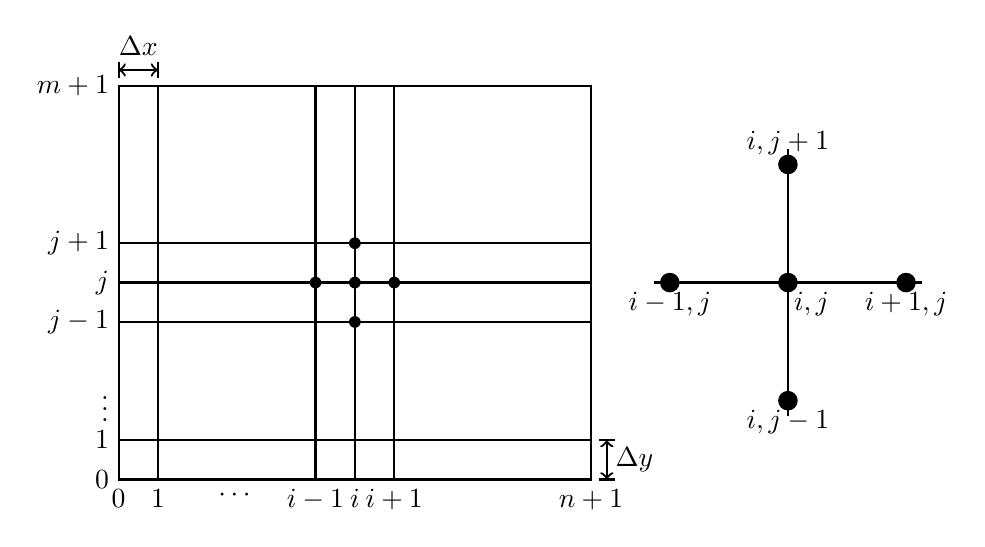
\begin{tikzpicture}




 
 
   

 \draw [black, thick] (0,0) rectangle (6,5);


\draw [black, thick] (0.5,0) -- (0.5, 5) ;

 \draw [black, thick] (2.5,0) -- (2.5, 5) ;
 \draw [black, thick] (3,0) -- (3, 5) ;
 \draw [black, thick] (3.5,0) -- (3.5, 5) ;
 
  \draw [black, thick] (0,2) -- (6, 2) ;
 \draw [black, thick] (0,2.5) -- (6, 2.5) ;
 \draw [black, thick] (0,3) -- (6, 3) ;
  \draw [black, thick] (0,0.5) -- (6, 0.5) ;
  
\node [below] at (0, 0) {$0$};
\node [below] at (0.5, 0) {$1$};
\node [below] at (1.5, 0) {$\cdots$};
\node [below] at (2.5, 0) {$i-1$};
\node [below] at (3, 0) {$i$};
 \node [below] at (3.5, 0) {$i+1$};
 \node [below] at (6, 0) {$n+1$};
 
 
 
 \node [left] at (0, 0) {$0$};
\node [left] at (0, 0.5) {$1$};
\node [left] at (0, 1) {$\vdots$};
\node [left] at (0, 2) {$j-1$};
\node [left] at (0, 2.5) {$j$};
 \node [left] at (0, 3) {$j+1$};
  \node [left] at (0, 5) {$m+1$};
 
 
 
 
    \draw[<->, thick] (0,5.2) -- (0.5,5.2);
        \draw [thick] (0,5.1) -- (0,5.3);
\draw [thick] (0.5,5.1) -- (0.5,5.3);
    \node at (0.25, 5.5) { $\Delta x$};
    
       \draw[<->, thick] (6.2, 0) -- (6.2, 0.5);
        \draw [thick] (6.1,0) -- (6.3, 0);
\draw [thick] (6.1, 0.5) -- (6.3, 0.5);
       \node at (6.55, 0.25) { $\Delta y$};
       
       
        \node at (3, 2.5)[circle,fill,inner sep=1.5pt]{};
        \node at (3, 3)[circle,fill,inner sep=1.5pt]{};
        \node at (3, 2)[circle,fill,inner sep=1.5pt]{};
        \node at (3.5, 2.5)[circle,fill,inner sep=1.5pt]{};
        \node at (2.5, 2.5)[circle,fill,inner sep=1.5pt]{};
        
        
        
        \draw [thick] (6.8,2.5) -- (10.2,2.5);
        \draw [thick] (8.5,0.8) -- (8.5,4.2);
         \node at (8.5, 2.5)[circle,fill,inner sep=2.5pt]{};
         \node at (8.5, 1)[circle,fill,inner sep=2.5pt]{};
         \node at (8.5, 4)[circle,fill,inner sep=2.5pt]{};
         \node at (7, 2.5)[circle,fill,inner sep=2.5pt]{};
         \node at (10, 2.5)[circle,fill,inner sep=2.5pt]{};
         
          \node at (8.8, 2.5) [below] {$i,j$};
          
           \node at (8.5, 1) [below] {$i,j-1$};
           \node at (8.5, 4) [above] {$i,j+1$};
           
            \node at (7, 2.5) [below] {$i-1,j$};
            \node at (10, 2.5) [below] {$i+1,j$};
 
    \end{tikzpicture}

$\Delta x= \frac{L_x}{n+1}, \quad \Delta y= \frac{L_y}{m+1}, \quad 
x_i = i\Delta x, \quad y_j = j\Delta y$


\end{frame}


   


%-=-=-=-=-=-=-=-=-=-=-=-=-=-=-=-=-=-=-=-=-=-=-=-=
%	FRAME:
%-=-=-=-=-=-=-=-=-=-=-=-=-=-=-=-=-=-=-=-=-=-=-=-=
\begin{frame}{Approximation of differential operator }
Use central finite difference on each direction:
\begin{equation*}
	\left.\frac{\partial^{2} u}{\partial x^{2}}\right|_{i, j} \approx \frac{u_{i+1, j}-2 u_{i, j}+u_{i-1, j}}{\Delta x^{2}}
\end{equation*}

\begin{equation*}
	\left.\frac{\partial^{2} v}{\partial y^{2}}\right|_{i, j} \approx \frac{u_{i, j+1}-2 u_{i, j}+u_{i, j-1}}{\Delta y^{2}}
\end{equation*}


Five point stencil:
\begin{equation*}
	-\nabla^2 u_{ij} \approx -\frac{1}{\Delta x^2}\left(u_{i-1,j}-2u_{ij}+u_{i+1,j}\right) -
	 \frac{1}{\Delta y^2}\left(u_{i,j-1}-2u_{ij}+u_{i,j+1} \right)
\end{equation*}

In particular, $\Delta x = \Delta y = h$:
\begin{equation*}
	-\nabla^2 u_{ij} \approx -\frac{1}{h^2}\left(u_{i-1,j}+u_{i,j-1}-4u_{ij}+u_{i+1,j}+u_{i,j+1} \right)
\end{equation*}

\end{frame}
   




%-=-=-=-=-=-=-=-=-=-=-=-=-=-=-=-=-=-=-=-=-=-=-=-=
%	FRAME:
%-=-=-=-=-=-=-=-=-=-=-=-=-=-=-=-=-=-=-=-=-=-=-=-=
\begin{frame}{Equations}


$-u_{x x}-u_{y y}=f$ suggests:
\begin{equation*}
	-\frac{u_{i+1, j}-2 u_{i, j}+u_{i-1, j}}{\Delta x^{2}}-\frac{u_{i, j+1}-2 u_{i, j}+u_{i, j-1}}{\Delta y^{2}}=f_{i, j}
\end{equation*}

\begin{equation*}
\begin{gathered}
u_{0, j}=g_D(x_0, y_j), u_{n+1, j}=g_D(x_{n+1}, y_j) \quad 1 \leq j \leq m \\
u_{i, 0}=g_D(x_i, y_0), u_{i, m+1}=g_D(x_i, y_{m+1}) \quad 1  \leq i \leq n \\
\Rightarrow \quad A \vec{u}=\vec{f}
\end{gathered}
\end{equation*}
 
\end{frame}
   

%-=-=-=-=-=-=-=-=-=-=-=-=-=-=-=-=-=-=-=-=-=-=-=-=
%	FRAME:
%-=-=-=-=-=-=-=-=-=-=-=-=-=-=-=-=-=-=-=-=-=-=-=-=
\begin{frame}{Example of Poisson equation in 2D }

\begin{columns}
\begin{column}{.4\textwidth}
\begin{equation*}
	m = n = 3
\end{equation*}
\begin{equation*}
	\Delta x = \Delta y = h
\end{equation*}


\end{column}

\begin{column}{.6\textwidth}
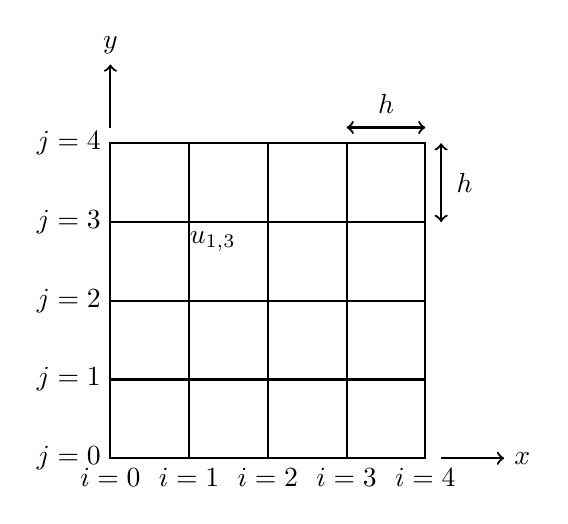
\begin{tikzpicture}




 
 
   

 \draw [black, thick] (0,0) rectangle (4,4);
\draw[->, thick] (4.2, 0) -- (5, 0) node[right] { $x$};
\draw[->, thick] (0, 4.2) -- (0, 5) node[above] { $y$};

    
\draw [thick] (1,0) -- (1, 4);
\draw [thick] (2,0) -- (2, 4);
\draw [thick] (3,0) -- (3, 4);   
    
\draw [thick] (0,1) -- (4, 1);
\draw [thick] (0,2) -- (4,2);
\draw [thick] (0,3) -- (4,3);   

    \node [below] at (0, 0) {$i=0$};
\node [below] at (1, 0) {$i=1$};
\node [below] at (2, 0) {$i=2$};
\node [below] at (3, 0) {$i=3$};
 \node [below] at (4, 0) {$i=4$};
 
 
 
 \node [left] at (0, 0) {$j=0$};
\node [left] at (0, 1) {$j=1$};
\node [left] at (0, 2) {$j=2$};
 \node [left] at (0, 3) {$j=3$};
  \node [left] at (0, 4) {$j=4$};
 
     \draw[<->, thick] (4.2,3) -- (4.2,4);
  \node at (4.5, 3.5) {$h$};
    
       \draw[<->, thick] (3, 4.2) -- (4, 4.2);
  \node at ( 3.5, 4.5) { $h$};
 
 
 
   \node at (1.3, 3) [below] {$u_{1,3}$};
    \end{tikzpicture}
 



\end{column}

\end{columns}

\end{frame}



%-=-=-=-=-=-=-=-=-=-=-=-=-=-=-=-=-=-=-=-=-=-=-=-=
%	FRAME:
%-=-=-=-=-=-=-=-=-=-=-=-=-=-=-=-=-=-=-=-=-=-=-=-=
\begin{frame}{Numbering scheme  }


\begin{columns}
\begin{column}{.5\textwidth}
   Natural rowwise ordering
\vspace{1em}


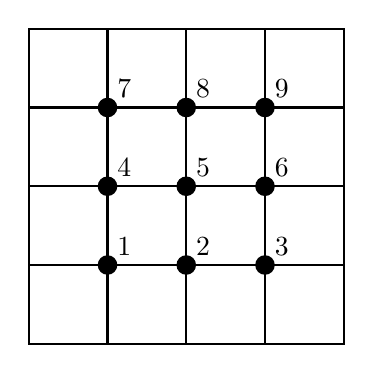
\begin{tikzpicture} 
   



 \draw [black, thick] (0,0) rectangle (4,4);

    
\draw [thick] (1,0) -- (1, 4);
\draw [thick] (2,0) -- (2, 4);
\draw [thick] (3,0) -- (3, 4);   
    
\draw [thick] (0,1) -- (4, 1);
\draw [thick] (0,2) -- (4,2);
\draw [thick] (0,3) -- (4,3);   

   \node at (1, 1)[circle,fill,inner sep=2.5pt]{};
   \node at (1, 2)[circle,fill,inner sep=2.5pt]{};
   \node at (1, 3)[circle,fill,inner sep=2.5pt]{};
    \node at (2, 1)[circle,fill,inner sep=2.5pt]{};
   \node at (2, 2)[circle,fill,inner sep=2.5pt]{};
   \node at (2, 3)[circle,fill,inner sep=2.5pt]{};
    \node at (3, 1)[circle,fill,inner sep=2.5pt]{};
   \node at (3, 2)[circle,fill,inner sep=2.5pt]{};
   \node at (3, 3)[circle,fill,inner sep=2.5pt]{};


 \node at (1, 1) [above right] {$1$};
\node at (2, 1) [above right]  {$2$};
\node at (3, 1) [above right]  {$3$};
 \node at (1, 2) [above right] {$4$};
\node at (2, 2) [above right]  {$5$};
\node at (3, 2) [above right]  {$6$};
 \node at (1, 3) [above right] {$7$};
\node at (2, 3) [above right]  {$8$};
\node at (3, 3) [above right]  {$9$};
    \end{tikzpicture}

\end{column}

\begin{column}{.5\textwidth}

Red-black ordering

\vspace{1em}



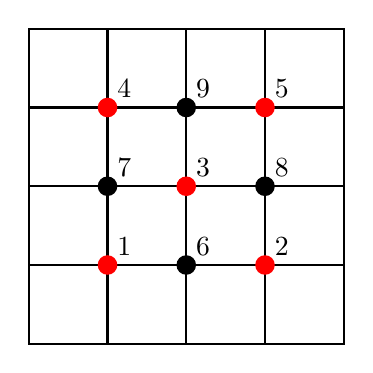
\begin{tikzpicture} 
   

 \draw [black, thick] (0,0) rectangle (4,4);

    
\draw [thick] (1,0) -- (1, 4);
\draw [thick] (2,0) -- (2, 4);
\draw [thick] (3,0) -- (3, 4);   
    
\draw [thick] (0,1) -- (4, 1);
\draw [thick] (0,2) -- (4,2);
\draw [thick] (0,3) -- (4,3);   


   \node at (1, 1)[circle, red, fill,inner sep=2.5pt]{};
   \node at (1, 2)[circle,fill,inner sep=2.5pt]{};
   \node at (1, 3)[circle, red, fill,inner sep=2.5pt]{};
    \node at (2, 1)[circle,fill,inner sep=2.5pt]{};
   \node at (2, 2)[circle, red, fill,inner sep=2.5pt]{};
   \node at (2, 3)[circle,fill,inner sep=2.5pt]{};
    \node at (3, 1)[circle, red, fill,inner sep=2.5pt]{};
   \node at (3, 2)[circle,fill,inner sep=2.5pt]{};
   \node at (3, 3)[circle,red, fill,inner sep=2.5pt]{};
 


 \node at (1, 1) [above right] {$1$};
\node at (2, 1) [above right]  {$6$};
\node at (3, 1) [above right]  {$2$};
 \node at (1, 2) [above right] {$7$};
\node at (2, 2) [above right]  {$3$};
\node at (3, 2) [above right]  {$8$};
 \node at (1, 3) [above right] {$4$};
\node at (2, 3) [above right]  {$9$};
\node at (3, 3) [above right]  {$5$};

    \end{tikzpicture}
 



\end{column}

\end{columns}
 
\end{frame}
   
   
   
   
  %-=-=-=-=-=-=-=-=-=-=-=-=-=-=-=-=-=-=-=-=-=-=-=-=
%	FRAME:
%-=-=-=-=-=-=-=-=-=-=-=-=-=-=-=-=-=-=-=-=-=-=-=-=
\begin{frame}{Equation at internal points -- natural rowwise ordering}

Eqn.1: $\quad -\frac{1}{h^{2}}\left(-4 u_{1}+u_{2}+u_{4}\right)=f_{1,1}+\frac{u_{0,1}+u_{1,0}}{h^{2}}$


Eqn.2: $\quad -\frac{1}{h^{2}}\left(u_{1}-4 u_{2}+u_{3}+u_{5}\right)=f_{2,1}+\frac{u_{2,0}}{h^{2}}$


Eqn.3: $\quad -\frac{1}{h^{2}}\left(u_{2}-4 u_{3}+u_{6}\right)=f_{3,1}+\frac{u_{3,0}+u_{4,1}}{h^{2}}$


Eqn.4: $\quad -\frac{1}{h^{2}}\left(u_{1}-4 u_{4}+u_{5}+u_{7}\right)=f_{1,2}+\frac{u_{0,2}}{h^{2}}$



Eqn.5: $\quad -\frac{1}{h^{2}}\left(u_{2}+u_{4}-4 u_{5}+u_{6}+u_{8}\right)=f_{2,2}$


Eqn.6: $\quad -\frac{1}{h^{2}}\left(u_{3}+u_{5}-4 u_{6}+u_{9}\right)=f_{3,2}+\frac{u_{4,2}}{h^{2}}$


Eqn.7: $\quad -\frac{1}{h^{2}}\left(u_{4}-4 u_{7}+u_{8}\right)=f_{13}+\frac{u_{0,3}+u_{1,4}}{h^{2}}$


Eqn.8: $\quad -\frac{1}{h^{2}}\left(u_{5}+u_{7}-4 u_{8}+u_{9}\right)=f_{2,3}+\frac{u_{2,4}}{h^{2}}$


Eqn.9: $\quad -\frac{1}{h^{2}}\left(u_{6}+u_{8}-4 u_{9}\right)=f_{33}+\frac{u_{3,4}+u_{4,3}}{h^{2}}$.


\end{frame}
   

%-=-=-=-=-=-=-=-=-=-=-=-=-=-=-=-=-=-=-=-=-=-=-=-=
%	FRAME:
%-=-=-=-=-=-=-=-=-=-=-=-=-=-=-=-=-=-=-=-=-=-=-=-=
\begin{frame}{Example: matrix and vector -- natural rowwise ordering}

\begin{equation*}
	A=\frac{1}{h^{2}}\left[\begin{array}{rrr|rrr|rrr}
4 & -1 & & -1 & & & & & \\
-1 & 4 & -1 & & -1 & & & & \\
& -1 & 4 & & & -1 & & & \\
\hline-1 & & & 4 & -1 & & -1 & & \\
& -1 & & -1 & 4 & -1 & & -1 & \\
& & -1 & & -1 & 4 & & & -1 \\
\hline & & & -1 & & & 4 & -1 & \\
& & & & -1 & & -1 & 4 & -1 \\
& & & & & -1 & & -1 & 4
\end{array}\right]
\end{equation*}


Assume $g_D=0$, we have 

$$ f = (f_{1,1}, f_{2,1},  f_{3,1}, f_{1,2}, f_{2,2},  f_{3,2}, f_{1,3}, f_{2,3},  f_{3,3})^T $$
 
\end{frame}
      
      
      
      
\begin{frame}{General finite difference method}
\begin{equation*}
-\frac{1}{\Delta y^2}u_{i,j-1}  -\frac{1}{\Delta x^2}u_{i-1,j} + 2\left(\frac{1}{\Delta x^2}+\frac{1}{\Delta y^2}\right)u_{i,j} 
-\frac{1}{\Delta x^2}u_{i+1,j}  -\frac{1}{\Delta y^2}u_{i,j+1} = f_{i,j}.
\end{equation*}



Let $\vec{u}_j = \left(u_{1,j}, u_{2,j}, \cdots, u_{n,j} \right)^T$
for $1\le j \le m$.



Rewrite as 
\begin{equation*}
D \vec{u}_{j-1} + C \vec{u}_j + D\vec{u}_{j+1} = \vec{f}_j;
\end{equation*}
where
{\small
\begin{equation*}
C =
\begin{bmatrix}
 2\left(\frac{1}{\Delta x^2}+\frac{1}{\Delta y^2}\right)& -\frac{1}{\Delta x^2}& & & &\\
-\frac{1}{\Delta x^2}& 2\left(\frac{1}{\Delta x^2}+\frac{1}{\Delta y^2}\right)& -\frac{1}{\Delta x^2}&&&\\
& \ddots & \ddots & \ddots& &&\\
&&-\frac{1}{\Delta x^2}& 2\left(\frac{1}{\Delta x^2}+\frac{1}{\Delta y^2}\right)& -\frac{1}{\Delta x^2}\\
&&&-\frac{1}{\Delta x^2}&2\left(\frac{1}{\Delta x^2}+\frac{1}{\Delta y^2}\right)
\end{bmatrix}
\end{equation*}
}
\end{frame}





      

%-=-=-=-=-=-=-=-=-=-=-=-=-=-=-=-=-=-=-=-=-=-=-=-=
%	FRAME:
%-=-=-=-=-=-=-=-=-=-=-=-=-=-=-=-=-=-=-=-=-=-=-=-=
\begin{frame}{General finite difference method (Continue)}
\begin{equation*}
D = 
\begin{bmatrix}
 -\frac{1}{\Delta y^2}& & & &\\
&-\frac{1}{\Delta y^2}& \\
&& \ddots & &&\\
&&& -\frac{1}{\Delta y^2}\\
&&&&-\frac{1}{\Delta y^2}
\end{bmatrix},
\vec{f}_j = 
\begin{pmatrix}
f_{1,j} +  \frac{1}{\Delta x^2}g_D(x_0, y_j)\\
 f_{2,j}\\ 
 \vdots\\
 f_{n-1,j}\\
  f_{n,j} + \frac{1}{\Delta x^2}g_D(x_{n+1}, y_j).
\end{pmatrix}
\end{equation*}


$C, D: (n\times n)$ 

 
\end{frame}







%-=-=-=-=-=-=-=-=-=-=-=-=-=-=-=-=-=-=-=-=-=-=-=-=
%	FRAME:
%-=-=-=-=-=-=-=-=-=-=-=-=-=-=-=-=-=-=-=-=-=-=-=-=
\begin{frame}{Linear system}

\begin{equation*}
A\vec{u} =
\begin{bmatrix}
 C& D& & &\\
 D&C&D& &\\
 & \ddots&\ddots&\ddots& \\
 &&D&C&D\\
 &&&D&C
\end{bmatrix}
\begin{pmatrix}
\vec{u}_1\\
\vec{u}_2\\
\vdots\\
\vec{u}_{m-1}\\
\vec{u}_m\\
\end{pmatrix}
=
\begin{pmatrix}
\vec{f}_1-D\vec{u}_{0}\\
\vec{f}_2\\
\vdots\\
\vec{f}_{m-1}\\
\vec{f}_m-D\vec{u}_{m+1}\\
\end{pmatrix}.
\end{equation*}

A:  \alert{Block} $(m\times m)$ tridiagonal matrix.
 
\end{frame}






%-=-=-=-=-=-=-=-=-=-=-=-=-=-=-=-=-=-=-=-=-=-=-=-=
%	FRAME:
%-=-=-=-=-=-=-=-=-=-=-=-=-=-=-=-=-=-=-=-=-=-=-=-=
\begin{frame}{Implementation of 2D FDM}
 \alert{Kronecker product }:  If $S$ is a $m\times n$ matrix and $T$ is a $p\times q$ matrix, then the Kronecker product of $S$ and $T$ is 
 $mp\times nq$ given by 
 \begin{equation*}
 S\otimes T = \begin{pmatrix}
s_{11}T &\cdots &s_{1n}T\\
\vdots & & \\
s_{m1}T &\cdots &s_{mn}T
\end{pmatrix}.
 \end{equation*}


 
\end{frame}











%-=-=-=-=-=-=-=-=-=-=-=-=-=-=-=-=-=-=-=-=-=-=-=-=
%	FRAME:
%-=-=-=-=-=-=-=-=-=-=-=-=-=-=-=-=-=-=-=-=-=-=-=-=
\begin{frame}{Implementation of 2D FDM (Continue)}
 
 Using Kronecker product, we can see that 
\begin{equation*}
A = \begin{bmatrix}
 C&& & &\\
 &C&& &\\
 & \ddots&\ddots&\ddots& \\
 &&&C&\\
 &&&&C
\end{bmatrix}  
+ 
\begin{bmatrix}
 O&D& & & &\\
 D&O&D& &\\
 & \ddots&\ddots&\ddots& \\
 &&D&O&D\\
 &&&D&O
\end{bmatrix}
= I_m\otimes C + E\otimes D;
\end{equation*}
where $I_m$ is the $m\times m$ identities matrix  and 
\begin{equation*}
E = 
\begin{bmatrix}
 0& 1& & & \\
1& 0& 1&&\\
&\ddots & \ddots & \ddots& &\\
&&1&0&1\\
&&&1&0
\end{bmatrix}.
\end{equation*}


In Matlab, you can use the function \alert{kron(S, T)} to compute $S\otimes T$.

 
\end{frame}






%-=-=-=-=-=-=-=-=-=-=-=-=-=-=-=-=-=-=-=-=-=-=-=-=
%	FRAME:
%-=-=-=-=-=-=-=-=-=-=-=-=-=-=-=-=-=-=-=-=-=-=-=-=
\begin{frame}{Truncation error}

$$
\begin{gathered}
-\frac{u\left(x_{i+1}, y_{j}\right)-2 u\left(x_{i}, y_{j}\right)+u\left(x_{i-1}, y_{j}\right)}{\Delta x^{2}} \\
-\frac{u\left(x_{i}, y_{j+1}\right)-2 u\left(x_{i}, y_{j}\right)+u\left(x_{i}, y_{j-1}\right)}{\Delta y^{2}}=f\left(x_{i}, y_{j}\right) \\
\underbrace{-\frac{\Delta x^{2}}{12} \frac{\partial^{4} u}{\partial x^{4}}\left(x_{i}+\theta_{i}^{x} \Delta x, y_{j}\right)-\frac{\Delta y^{2}}{12} \frac{\partial^{4} u}{\partial y^{4}}\left(x_{i}, y_{j}+\theta_{j}^{y} \Delta y\right)}_{\tau_{i, j}}
\end{gathered}
$$
For $u \in \mathcal{C}^{4}$, $\tau_{i, j} \sim \mathcal{O}\left(\Delta x^{2}, \Delta y^{2}\right) \quad$ for all $i, j$
	
\end{frame}




%-=-=-=-=-=-=-=-=-=-=-=-=-=-=-=-=-=-=-=-=-=-=-=-=
%	FRAME:
%-=-=-=-=-=-=-=-=-=-=-=-=-=-=-=-=-=-=-=-=-=-=-=-=
\begin{frame}{Convergence }

 Original scheme
 \[  A  \vec{u} = \vec{f}.  \]

 \vspace{0.2em}
 

Consistency 
\[ A  \hat{{u}} = \vec{f} + \vec{\tau}. \]

 \vspace{0.2em}


Error equation

\[
\mathbf{E} =  -A^{-1}\vec{\tau}.
\]

Taking norms
\begin{align*}
	\|\mathbf{E}\| =  &\| -A^{-1}\vec{\tau}\|\\
	               \le & \|A^{-1}\|\|\vec{\tau}\|\\
	               \le & \|A^{-1}\|Ch^2. 
\end{align*}


\end{frame}




%-=-=-=-=-=-=-=-=-=-=-=-=-=-=-=-=-=-=-=-=-=-=-=-=
%	FRAME:
%-=-=-=-=-=-=-=-=-=-=-=-=-=-=-=-=-=-=-=-=-=-=-=-=
\begin{frame}{ Recap of FD Methods}


   
Easy for simple geometry e.g. rectangles.

\vspace{1em}

Convergence theory can be tricky.


\vspace{1em}


 Produces large sparse matrices, even in 2D.

	
\end{frame}




%-=-=-=-=-=-=-=-=-=-=-=-=-=-=-=-=-=-=-=-=-=-=-=-=
%	FRAME:
%-=-=-=-=-=-=-=-=-=-=-=-=-=-=-=-=-=-=-=-=-=-=-=-=
\begin{frame}{ Other topics}


   
 Curved Regions also make finite difference methods messy, but possible.  See for example  `Immersed Interface Method' Ref: Li \& Leveque 1994.


\vspace{1em}

 Nonlinear elliptic PDEs can be tackled by  quasi-linearisation or by Newton's method and its variants

\vspace{1em}


For easy problems ($-\nabla^2u=f$) on a square there are special `fast Poisson solvers' that don't generalize to the variable coefficient case, or other coordinate systems.


	
\end{frame}




%-=-=-=-=-=-=-=-=-=-=-=-=-=-=-=-=-=-=-=-=-=-=-=-=
%	FRAME:
%-=-=-=-=-=-=-=-=-=-=-=-=-=-=-=-=-=-=-=-=-=-=-=-=
\begin{frame}{ 9-point stenicl}

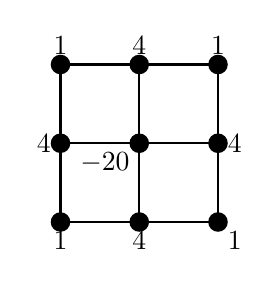
\begin{tikzpicture}

 \draw [black, thick] (0,0) rectangle (2,2);

\draw [black, thick](1, 0) -- (1,2);
\draw [black, thick](0, 1) -- (2, 1);
       
        
         \node at (0, 0)[circle,fill,inner sep=2.5pt]{};
         \node at (1, 0)[circle,fill,inner sep=2.5pt]{};
         \node at (2, 0)[circle,fill,inner sep=2.5pt]{};
\node at (0, 1)[circle,fill,inner sep=2.5pt]{};
         \node at (1, 1)[circle,fill,inner sep=2.5pt]{};
         \node at (2, 1)[circle,fill,inner sep=2.5pt]{};
         
         \node at (0, 2)[circle,fill,inner sep=2.5pt]{};
         \node at (1, 2)[circle,fill,inner sep=2.5pt]{};
         \node at (2, 02)[circle,fill,inner sep=2.5pt]{};


 \node at (0, 0) [below ] {$1$};
          \node at (1, 0) [below ] {$4$};
          \node at (2, 0) [below right] {$1$};

          \node at (0, 1) [ left] {$4$};
          \node at (1, 1) [below left] {$-20$};
          \node at (2, 1) [right] {$4$};

 \node at (0, 2) [above ] {$1$};
          \node at (1, 2) [above ] {$4$};
          \node at (2, 2) [above ] {$1$};

          
         
\end{tikzpicture}

Finite difference scheme:

\begin{align*}
\nabla^2_9u_{ij}=&\frac{1}{6h^2}[4u_{i-1,j}+4u_{i+1,j}+4u_{i,j-1}+4u_{i,j+1}+\\&u_{i-1,j-1}+u_{i-1,j+1}+u_{i+1,j-1}+u_{i+1,j+1} - 20 u_{i,j}].
\end{align*}
	
\end{frame}








%-=-=-=-=-=-=-=-=-=-=-=-=-=-=-=-=-=-=-=-=-=-=-=-=
%	FRAME:
%-=-=-=-=-=-=-=-=-=-=-=-=-=-=-=-=-=-=-=-=-=-=-=-=
\begin{frame}{ Truncation error of 9-point stencil}

Compute: 
\begin{equation*}
\nabla^2_9u(x_i, y_j)=\nabla^2u+\underbrace{\frac{1}{12}h^2(u_{xxxx}+2u_{xxyy}+u_{yyyy})+O(h^4)}_{\mbox{\large$\tau_{ij}$}},
\end{equation*}
   

Reformulate:
\begin{align*}
\tau_{ij}=& \frac{1}{12}h^2\nabla^2(\nabla^2 u)+O(h^4)\\
&= - \frac{1}{12}h^2\nabla^2f+O(h^4).
\end{align*}


Observation: if we know $f$ analytically, we can evaluate the first term of $\tau_{ij}$.

\vspace{0.5em}

Example: $f=0$ then error is $O(h^4)$, \mbox{$\nabla^2_9u=0 \to A_9\vec{u}=\vec{b}$}, $\tau=O(h^4)$. 
	
\end{frame}



%-=-=-=-=-=-=-=-=-=-=-=-=-=-=-=-=-=-=-=-=-=-=-=-=
%	FRAME:
%-=-=-=-=-=-=-=-=-=-=-=-=-=-=-=-=-=-=-=-=-=-=-=-=
\begin{frame}{ 4th Order method for Poisson equation}
For Poisson equation:
 \[ -\nabla_9^2u=f+\frac{1}{12}h^2\nabla^2f  +O(h^4),\]
 
 
 
Consider \alert{different problem}:
 \[ -\nabla_9^2u=f+\frac{1}{12}h^2\nabla^2f=\tilde{f},\]
  then \[-\nabla^2u +\frac{1}{12}h^2\nabla^2\tilde{f}+O(h^4)=\tilde{f},\]
  therefore \[-\nabla^2u +\frac{1}{12}h^2\nabla^2f+O(h^4)=f+\frac{1}{12}h^2\nabla^2f,\]
   so
    \[-\nabla^2 u+O(h^4)=f,\]
    i.e. we've solved $-\nabla^2 u=f$ to $O(h^4)$.



	
\end{frame}




%-=-=-=-=-=-=-=-=-=-=-=-=-=-=-=-=-=-=-=-=-=-=-=-=
%	FRAME:
%-=-=-=-=-=-=-=-=-=-=-=-=-=-=-=-=-=-=-=-=-=-=-=-=
\begin{frame}{Unknown right hand side}
If we don't know $f$ analytically, but just at grid points. 
Just form 
\begin{align*}
\tilde{f}_{i,j}=&f_{i,j}+\frac{1}{12}h^2\nabla_5^2f_{i,j}\\
=&f_{i,j}+\frac{1}{12}h^2(\nabla^2f+O(h^2))\\
=&f_{i,j}+\frac{1}{12}h^2\nabla^2f_{i,j}+O(h^4),
\end{align*}
	
\end{frame}


%-=-=-=-=-=-=-=-=-=-=-=-=-=-=-=-=-=-=-=-=-=-=-=-=
%	FRAME:
%-=-=-=-=-=-=-=-=-=-=-=-=-=-=-=-=-=-=-=-=-=-=-=-=
\begin{frame}{Method of deferred corrections}


Solve $A_5{\vec{u}}=\vec{f}$ which  gives $\vec{u}$ with an error $O(h^2)$. We know 
\[ \tau_{ij} = \frac{1}{12}h^2(u_{xxxx}+u_{yyyy}) + O(h^4).\]

Then, since $A_5\hat{u}-\vec{f}=\tau$ and $A_5\vec{u}-\vec{f}=\vec{0}$, 
 \[ 
A_5(\vec{u}-\hat{u})=-\vec{\tau}
\Rightarrow
A_5 E = -\tau.
\]
We now attempt to use $\vec{u}$ to estimate $\tau$.
For example we can use central differences to get $u_{xxxx}$ and $u_{yyyy}$ to  $O(h^2)$. Then we obtain 
\[\hat{\tau} = \vec{\tau} +O(h^4),\] 
and solve 
\[A_5 E=-\hat{\tau},\] 
then update 
\[\tilde{\vec{u}}=\hat{\vec{u}}-{E},\] 
which has improved our estimate to $O(h^4)$.
\end{frame}



%-=-=-=-=-=-=-=-=-=-=-=-=-=-=-=-=-=-=-=-=-=-=-=-=
%	FRAME:
%-=-=-=-=-=-=-=-=-=-=-=-=-=-=-=-=-=-=-=-=-=-=-=-=
\begin{frame}[standout]
  End of week 5!
\end{frame}

\appendix



\end{document}
                                                                                  